\section{CAFE問題}

車両装備仕様問題は,\textbf{装備タイプ}とそれに付随する\textbf{装備オプション}から構成される.
装備タイプはエンジンやタイヤなどの装備の種類を表し,
装備オプションは,4気筒エンジン,15インチタイヤなどの具体的な装備を表す.
以降,装備タイプをタイプ,装備オプションをオプションと呼ぶことにする.


\textbf{装備仕様}とは,タイプとオプションの組合せであり,
(エンジン, 4気筒), (タイヤ, 15インチ)などの対の集合で表される.
車両装備仕様問題の目的は,与えられたタイプとオプションの集合から,
装備および燃費に関する制約を満たしつつ,販売台数を最大化する装備仕様を求める問題である.
本研究では,燃費に関する制約として,
企業別平均燃費 (Corporate Average Fuel Efficiency; CAFE)基準を採用する.
このCAFE基準は,自動車の燃費規制で,車種別ではなくメーカー全体で出荷台数を加味した
平均燃費を算出する方式である.日本では2020年度の燃費基準に採用されている.
以降では,CAFE基準による燃費制約を持つ車両装備仕様問題を\textbf{CAFE問題}と呼ぶ.

CAFE問題を表現する方法として,OVM(Orthogonal Variability Model)
\cite{Pohl05:sple}を用いる.図%\ref{fig:ovm_notation}
にOVMの表記法を示す.OVMでは,仕様ごとに変わりうる項目を
\textbf{可変点(Variation Point;VP)},その具体的なインスタンスを
\textbf{バリアント(Variant;V)}と呼ぶ.VPとVの対応関係には選択式(optional),
必須式(mondatory)があり,1つのVPに対して複数の選択式Vが存在する場合,
多重度によって制限された数のVが選択される.
また,VP間,V間,VPとV間に必要(require)や排除(exclude)の関係を定義することができる.

\begin{figure*}[t]
 \centerline {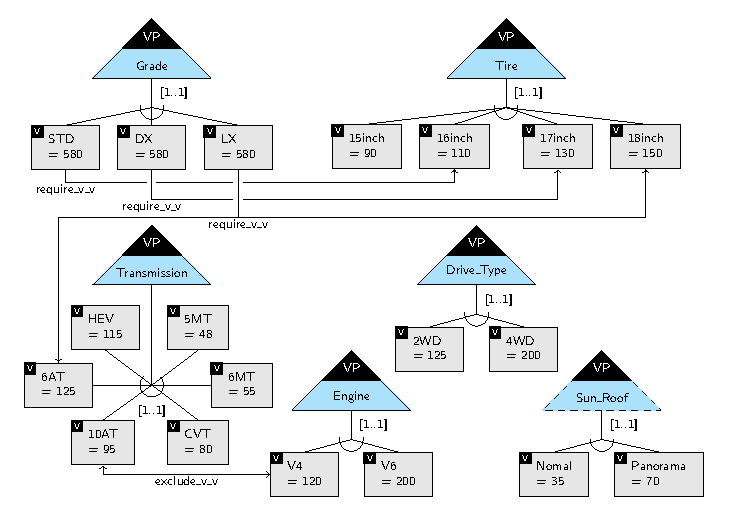
\includegraphics{images/ovm01.eps}}
 \caption{CAFE問題の例}
 \label{fig:ovm_example}
\end{figure*}

OVMで表現されたCAFE問題の例を図%\ref{fig:ovm_example}
に示す.CAFE問題においては,タイプがVP,オプションがVとして表現され,Vの多重度は
全て[1:1]で,各タイプごとにちょうど1つのオプションが選択される.
ただし,CAFE問題では図%ref{fig:ovm_example}
のSun\_Roofのような必須ではないタイプが存在し,この選択式のVPは点線で囲って表現する.
オプションにはIWRと呼ばれる重みのようなものがそれぞれ定められており,
装備仕様ごとに選択されるオプションのIWRの和を引数として,あらかじめ与えられている
テーブルにより燃費と予想販売台数を得ることができる.CAFE問題の燃費制約とは,
装備仕様ごとの出荷台数も加味した全体の平均燃費が与えられた\textbf{CAFE基準値}以上に
ならなければならないという制約である.3種類の装備仕様による燃費制約を式で表現すると,
装備仕様$i$の燃費を$Fe_i$,予想販売台数を$V_i$として,以下のようになる.
\vspace{1em}
 \begin{displaymath}
  %\label{eq:cafe1} 
   \underbrace{
   \frac{Fe_{1} \times V_1 + Fe_{2} \times V_2 + Fe_{3} \times V_3 }{V_1 + V_2 + V_3}
   }_{\mbox{平均燃費}}
   \geq 
   \underbrace{t}_{\mbox{CAFE基準値}}
  \end{displaymath}
\vspace{1em}

表\ref{tab:ovm_ans}
にて,図%\ref{fig:ovm_example}
に対する解の例を示す.このとき,求める装備仕様を3種類,CAFE基準値を9.0km/Lとする.
\begin{table}[tb]
 \caption{CAFE問題の解の例}
 \begin{tabular}{l|c|c|c} \bhline
    \multicolumn{1}{c|}{装備}   & \multicolumn{3}{c}{装備仕様} \\ \cline{2-4}
                 & 1	& 2 	 & 3	\\  \hline
    Grade	 & STD	& DX	 & LX	\\
    Drive\_Type  & 2WD  & 2WD    & 2WD  \\
    Engine	 & V4	& V6	 & V6	\\
    Tire	 & 16	& 17	 & 18	\\
    Transmission & 5MT	& 6MT    & 10AT	\\
    Sun\_Roof    & -    & normal & -    \\ \hline
    IWR          & 983  & 1125   & 1180 \\ %\hline
    燃費(km/L)    & 10.2  & 8.9     & 8.5 \\ %\hline
    予想販売台数  & 745  & 1988   & 1171  \\ \hline
    平均燃費(km/L) & \multicolumn{3}{c}{\bf{9.0}} \\ 
    合計販売台数  & \multicolumn{3}{c}{\bf{3904}} \\ \hline
 \end{tabular}
 \label{tab:ovm_ans}
\end{table}
各装備仕様の列に,それぞれのタイプで選択されるオプションが示されており,IWRの和から
燃費と予想販売台数が算出され,これらの値から全体の平均燃費と合計の販売台数が求められる.






% - CAFE問題の定義
% - OVMの解説
% - CAFE問題をOVMで表現
%   - 必須VPの説明どうする?既存のOVMにはない考え方
% - CAFE問題の各種制約をOVMになぞらえて解説
% - 解の例